\begin{enumerate}[label=\thesubsection.\arabic*,ref=\thesubsection.\theenumi]
    \item The Euler iteration formula for numerically integrating a first order nonlinear differential equation of form $x = f(x)$, with a constant step size of $\Delta t$ is 
	    \hfill (AE 2007)
    \begin{multicols}{2}
    \begin{enumerate}
        \item $x_{k+1} = x_k - \Delta t \times f(x_k)$ 
        \item $x_{k+1} = x_k + \left( \Delta t^2 / 2 \right) \times f(x_k)$ 
        \item $x_{k+1} = x_k - (1 / \Delta t) \times f(x_k)$ 
        \item $x_{k+1} = x_k + \Delta t \times f(x_k)$
    \end{enumerate}
    \end{multicols}
    \item Numerical values of the integral 
    $\int_{0}^{1} \frac{1}{1 + x^2}\,dx$ if evaluated numerically using the Trapazoidal rule with dx = 0.2 would be
    \hfill (AE 2007)
    \begin{multicols}{4}
\begin{enumerate}
        \item 1
        \item $\pi/4$
        \item 0.7837
        \item 0.2536
    \end{enumerate}
    \end{multicols}
    \item The Newton-Raphson iteration formula to find a cube root of a positive number $c$ is
    \hfill (AE 2007)
\begin{enumerate}
    \begin{multicols}{4}
        \item $x_{k+1} = \frac{2 x_k^3 + \sqrt[3]{c}}{3 x_k^2}$
        \item $x_{k+1} = \frac{2 x_k^3 - \sqrt[3]{c}}{-3 x_k^2}$
        \item $x_{k+1} = \frac{2 x_k^3 + c}{3 x_k^2}$
        \item $x_{k+1} = \frac{x_k^3 + c}{3 x_k^2}$
	\end{multicols}
    \end{enumerate}
\item 
$y(0) = 0$ and using Euler's method with step size $h = 0.1$ solution of the differential equation
\begin{align*}
\frac{dy}{dx} &= 2xy + 1
\end{align*}
gives the value of
$y(0.3)  =  $?
\hfill(AG 2007)
\begin{multicols}{4}
\begin{enumerate}
    \item 0.3101
    \item 0.3142
    \item 0.6202
    \item 4.080
\end{enumerate}
\end{multicols}
\item Integrating the function
\hfill(AG 2007)
\begin{align*}
f(x) &= 1 + e^{-x} \sin(4x)
\end{align*}
over the interval [0, 1] using Simpson's $\frac{1}{3}$ rule gives Result =  ?
\begin{multicols}{4}
\begin{enumerate}
    \item 1.021
    \item 1.091
    \item 1.321
    \item 2.642
\end{enumerate}
\end{multicols}
\item The degree of the differential equation $\frac{d^2x}{dt^2}+2x^3=0$ is
\hfill{\brak{\text{CE 2007}}}
\begin{multicols}{4}
\begin{enumerate}
\item 0
\item 1
\item 2
\item 3
\end{enumerate}
\end{multicols}

\item The solution of the differential equation $\frac{dy}{dx}=x^2y$ with the condition that $y=1$ at $x=0$ is
\hfill{\brak{\text{CE 2007}}}
\begin{multicols}{4}
\begin{enumerate}
\item $y=e^{\frac{1}{2x}}$
\item $\ln(y)=\frac{x^3}{3}+4$
\item $\ln(y)=\frac{x^2}{2}$
\item $y=e^{\frac{x^3}{3}}$
\end{enumerate}
\end{multicols}

\item The following equation needs to be numerically solved using the Newton-Raphson method. $x^3 + 4x - 9 = 0$
The iterative equation for this purpose is $\brak{\text{k indicates the iteration level}}$
\hfill{\brak{\text{CE 2007}}}
\begin{multicols}{2}
\begin{enumerate}
\item $x_{k+1} = \frac{2x_k^3 + 9}{3x_k^2 + 4}$
\item $x_{k+1} = \frac{2x_k^3 + 9}{3x_k^2 + 9}$
\item $x_{k+1} = x_k - \frac{x_k^3 + 4x_k - 9}{3x_k^2 + 4}$
\item $x_{k+1} = \frac{4x_k^2 + 3}{9x_k^2 + 2}$
\end{enumerate}
\end{multicols}

\item Given that one root of the equation $x^3 - 10x^2 + 31x - 30 = 0$ is 5, the other two roots are
\hfill{\brak{\text{CE 2007}}}
\begin{multicols}{4}
\begin{enumerate}
\item 2 and 3
\item 2 and 4
\item 3 and 4
\item -2 and -3
\end{enumerate}
\end{multicols}
    \item Consider the series $x_{n+1}=\frac{x_n}{2}+\frac{9}{8x_n},x_0=0.5$ obtained from the Newton-Raphson method. The series converges to
    \hfill {(CS 2007)}
    \begin{enumerate}
        \begin{multicols}{4}
        \item $1.5$
        \item $\sqrt{2}$
        \item $1.6$
        \item $1.4$
         \end{multicols}
    \end{enumerate}
\item The following plot shows a function $y$ which varies linearly with $x$. The value of the integral $\int_{0}^{2} y \, dx$ is:
\hfill{\brak{\text{EC 2007}}}

\begin{figure}[H]
    \centering
    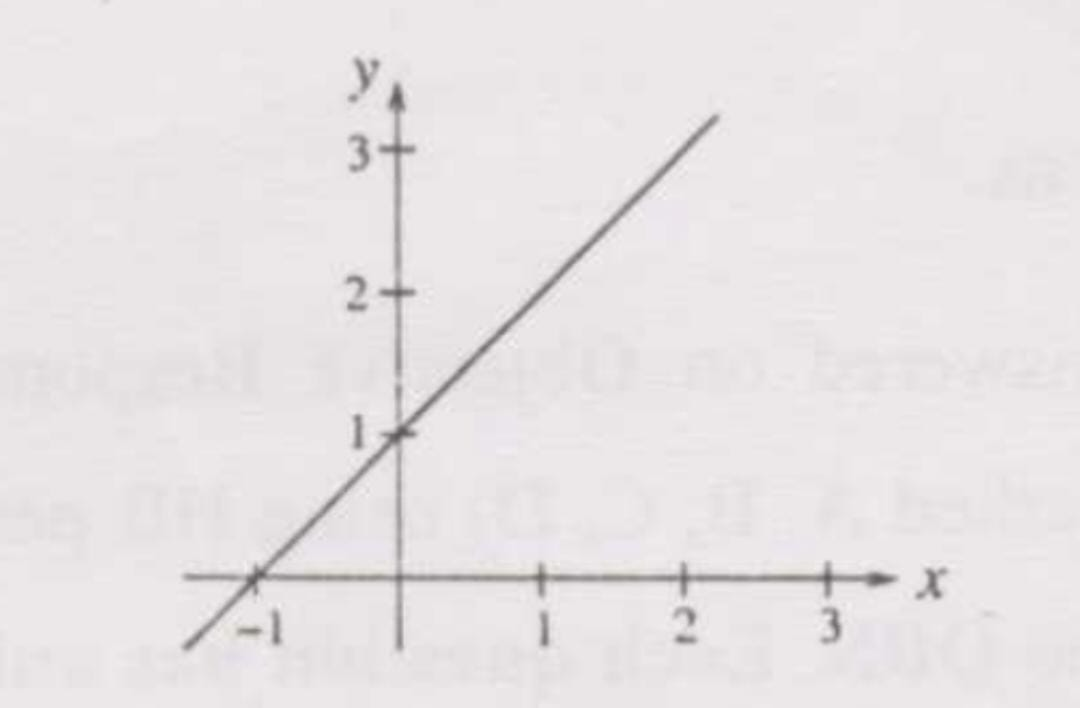
\includegraphics[width=0.4\textwidth]{figs/2007/EC/Q2.jpg}
    \caption{}
    \label{fig:Q2.jpg}
\end{figure}


\begin{enumerate}
\begin{multicols}{4}
    \item 1.0
    \item 2.5
    \item 4.0
    \item 5.0
\end{multicols} 
\end{enumerate}


\item For $|x| < 1 $, $ \coth(x)$ can be approximated as: 
\hfill{\brak{\text{EC 2007}}}
\begin{enumerate}
\begin{multicols}{4}
    \item $ x $
    \item $ x^2 $
    \item $ \frac{1}{x} $
    \item $ \frac{1}{x^2} $
\end{multicols} 
\end{enumerate}

\item $ \lim_{\theta \to 0} \frac{\sin(\theta/2)}{\theta} $ is: 
\hfill{\brak{\text{EC 2007}}}
\begin{enumerate}
\begin{multicols}{4}
    \item 0.5
    \item 1
    \item 2
    \item Not defined
\end{multicols} 
\end{enumerate}

\item Which of the following functions is strictly bounded? 
\hfill{\brak{\text{EC 2007}}}
\begin{multicols}{4}
\begin{enumerate}
    \item $ \sin x $
    \item $ e^x $
    \item $ \cos x $
    \item $ x^2 $
\end{enumerate}
\end{multicols}

\item For the function $ e^{-x} $, the linear approximation around $ x = 2 $ is:
\hfill{\brak{\text{EC 2007}}}
\begin{enumerate}
    \item $ (3 - x)^2 $
    \item $ 1 - x $
    \item $ [3 + 2\sqrt{2} - (1 + \sqrt{2})x]e^2 $
    \item $ e^{-2} $
\end{enumerate}

\item The equation $x^2 + x^4 - 4x - 4 = 0$ is to be solved using Newton-Raphson. If $x = 2$ is the initial approximation, then the next approximation using this method will be:
\hfill{\brak{\text{EC 2007}}}

\begin{multicols}{4}
\begin{enumerate}
    \item $\frac{2}{3}$
    \item $\frac{4}{3}$
    \item $1$
    \item $\frac{3}{2}$   
\end{enumerate}
\end{multicols}
\item
A 5-point sequence $x[n]$ is given as $x[-3]=1$, $x[-2]=1$, $x[-1]=0,
x[0]=5$, $x[1]=15$. Let $X\left(e^{j\omega}\right)$ denote the discrete-time Fourier
transform of $x[n]$. The value of
$
\int_{-\pi}^{\pi} X\left(e^{4j\omega3}\right)\, d\omega
$
\hfill{\brak{\text{EC 2007}}}
\begin{multicols}{4}
\begin{enumerate}
  \item 5
  \item $10\pi$
  \item $16\pi$
  \item $5 + j10\pi$
\end{enumerate}
\end{multicols}

\item The $z$-transform $X[z]$ of a sequence $x[n]$ is given by
$
X[z]=\frac{0.5}{1-2z^{-1}}.
$
It is given that the region of convergence of $X[z]$ includes the unit circle. The value of $x[0]$ is: 
\hfill{\brak{\text{EC 2007}}}
\begin{multicols}{4}
\begin{enumerate}
    \item $-0.5$
    \item $0$
    \item $0.25$
    \item $0.5$
\end{enumerate}
\end{multicols}

\end{enumerate}

